\documentclass[12pt]{article}
\usepackage{geometry}
\usepackage{graphicx}
\usepackage{amsmath}
\usepackage{fancyhdr}
\usepackage{hyperref}
\usepackage{booktabs}    % For professional-looking tables
\usepackage{array}       % For extended column definitions
\usepackage{tabularx}    % For adjustable-width tables
\usepackage{longtable}

\geometry{margin=1in}
\hypersetup{
	colorlinks=true,  % Set to true to use colored text for links
	linkcolor=blue,   % Set the color for internal links (e.g., table of contents)
	urlcolor=blue,    % Set the color for external links
	citecolor=blue,   % Set the color for citations
	pdfborder={0 0 0} % Remove the border around links
}
\title{Aircraft Design 1 - Fall 2024 \\ Assignment 2}
\author{Smythe Cy Goforth Jr, Matthew Burnett \\ Group 6 \\ Instance: [first delivery]}
\date{Hours spent on assignment: [60]}

\begin{document}
	
	\maketitle
	\newpage
	
	
	\begin{figure}[h!]
		\centering
		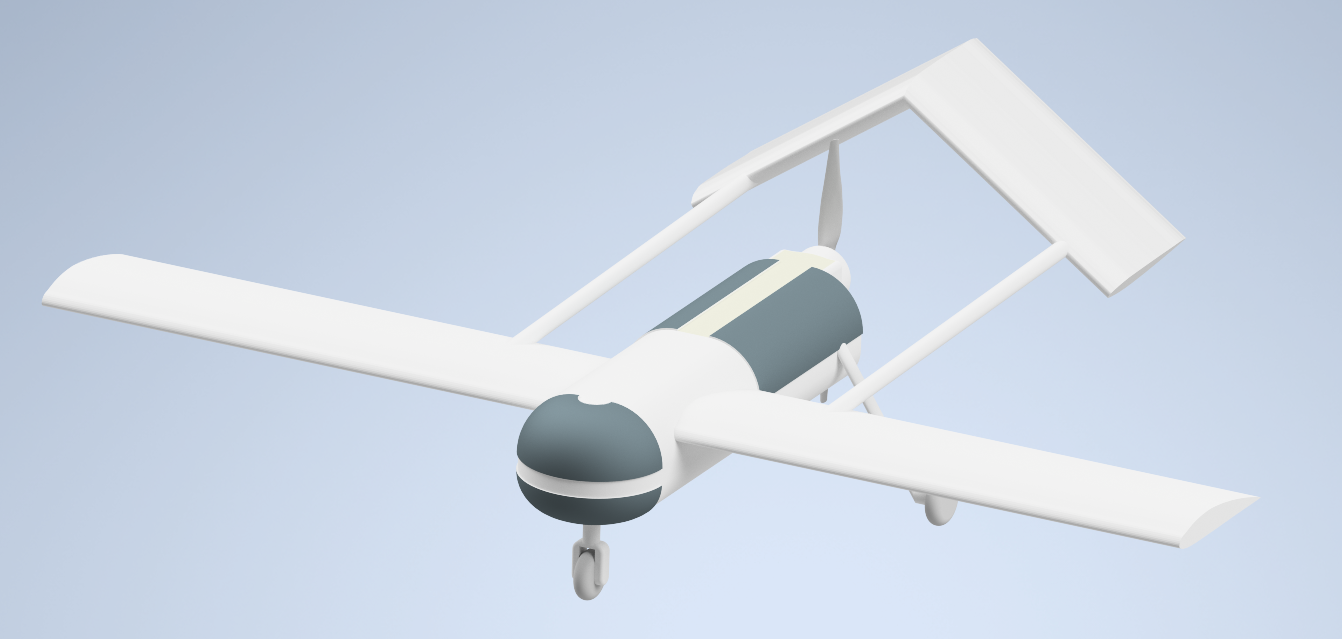
\includegraphics[width=6 in]{Figures/Drone.png} % Placeholder for technical drawings
		\caption{Rendered design of the LAHE UAV}
	\end{figure}
	
	\newpage
	
	\tableofcontents
	
	\newpage
	\section{Introduction}
	
	This report is divided into two main parts. The first part focuses on the preliminary sizing of a UAV, using data from reference aircraft and the specific design requirements. It includes the estimation of takeoff weight, the creation of the W/P–W/S diagram, and the generation of the drag polar. Additionally, it explores the optimal takeoff weight in relation to the payload-range diagram.
	
	The second part addresses the propulsion system, proposing a selection of motors based on the required thrust under various weight conditions. The analysis includes engine type, weight, and dimensions, followed by scaling to meet the UAV’s specific requirements. The report also covers optimization of the motor’s thermodynamic cycle and energy expenditure, with validation of the selected design values. All weights in this report are expressed in kilograms at sea level, defined as:
	
	\[
	W_{\text{Kg}_\text{sea level}} = \frac{W_{\text{newtons}}}{9.81~m/s^2}
	\]

		
	\section{Determining the Takeoff Weight}
	To determine the takeoff weight (\(W_{TO}\)), various components of the overall aircraft weight must be identified. The takeoff weight typically consists of operational empty weight (\(W_{OE}\)), fuel weight (\(W_{Battery}\)), and payload weight (\(W_{Payload}\)). In our case, as the aircraft is a battery-powered UAV, the fuel weight is exclusively the weight of the onboard batteries. Therefore, this chapter will calculate the fuel weight based on two different battery configurations outlined in Assignment 1. The battery weight is inversely proportional to the payload weight, leading to two separate payload configurations. Since batteries are static and installed prior to flight they are enveloped under operational empty weight.
	
	The total takeoff weight can be calculated using the equation:
	
	\begin{equation}
		W_{TO} = W_{Payload} + W_{OE} \tag{Eq 2.1}
	\end{equation}
	
	\subsection{Payload}
	The payload is defined as the total weight of all components of the sensor package deployed with the UAV. Based on reference aircraft, the estimated payload weight is approximately \(6.60 \text{ kg}\). Due to the aircraft's design, which allows for battery space to be exchanged for additional payload space, a secondary payload configuration can be implemented. This configuration involves removing one of the two batteries, resulting in a payload weight increase.
	\begin{enumerate}
		\item Endurance Configuration Payload Mass: \(6.60 \text{ kg}\) 
		\item Heavy Lift Configuration Payload Mass: \(10.60 \text{ kg}\)
	\end{enumerate}

	
	
	\subsection{Batteries}
	In contrast to hydrocarbon-powered aircraft, where fuel weight comprises both used and reserve fuel, the fuel weight for electric aircraft is solely determined by the battery pack weight. The weight of these battery packs remains constant throughout the flight. For our UAV, two battery configurations are considered: using one or two \(40 \text{ Ah}\) batteries, each weighing approximately \(4 \text{ kg}\).

	
	
	\subsection{Operational Empty Weight}
	The operational empty weight (\(W_{OE}\)) can be determined using the following equation:
	
	\begin{equation}
		W_{OE} = W_{E} + W_{Battery}
	\end{equation}
	
	to expand empty weight ($W_{E}$) further:
	
	\begin{equation}
		W_{OE} = W_{Fuselage} + W_{Avioncis} + W_{Motor} + W_{Battery}
	\end{equation}
	
	with the following approximate values the operational empty weight can be estimated:
	
	\begin{equation}
		W_{OE} = 12\text{ Kg} + 4\text{ Kg} + 1\text{ Kg} + 8\text{ Kg}
	\end{equation}
	\begin{equation}
		W_{OE} = 25\text{ Kg}
	\end{equation}
		
	The estimations for fuselage weight was derived from the CAD assuming fiber glass construction, as the current model of the fuselage is considerably over built, this weight is likely an over-estimation. The motor and avionics weight was estimated from data sheets of typical components needed for UAV's of this scale. The battery weight was also gathered from data sheets, all operating on the same chemistry, the battery wieghts for 24 V 40,000 mAh LiPO batteries was almost identical.
	
	Using reference aircraft data a maximum payload and a maximum take off weight (MTOW) can be estimated. Payload and empty take off weight (ETOW) data for refrence aircraft was plotted and a quadratic curve was fitted.
	
	\begin{figure}[h!]
	\centering
		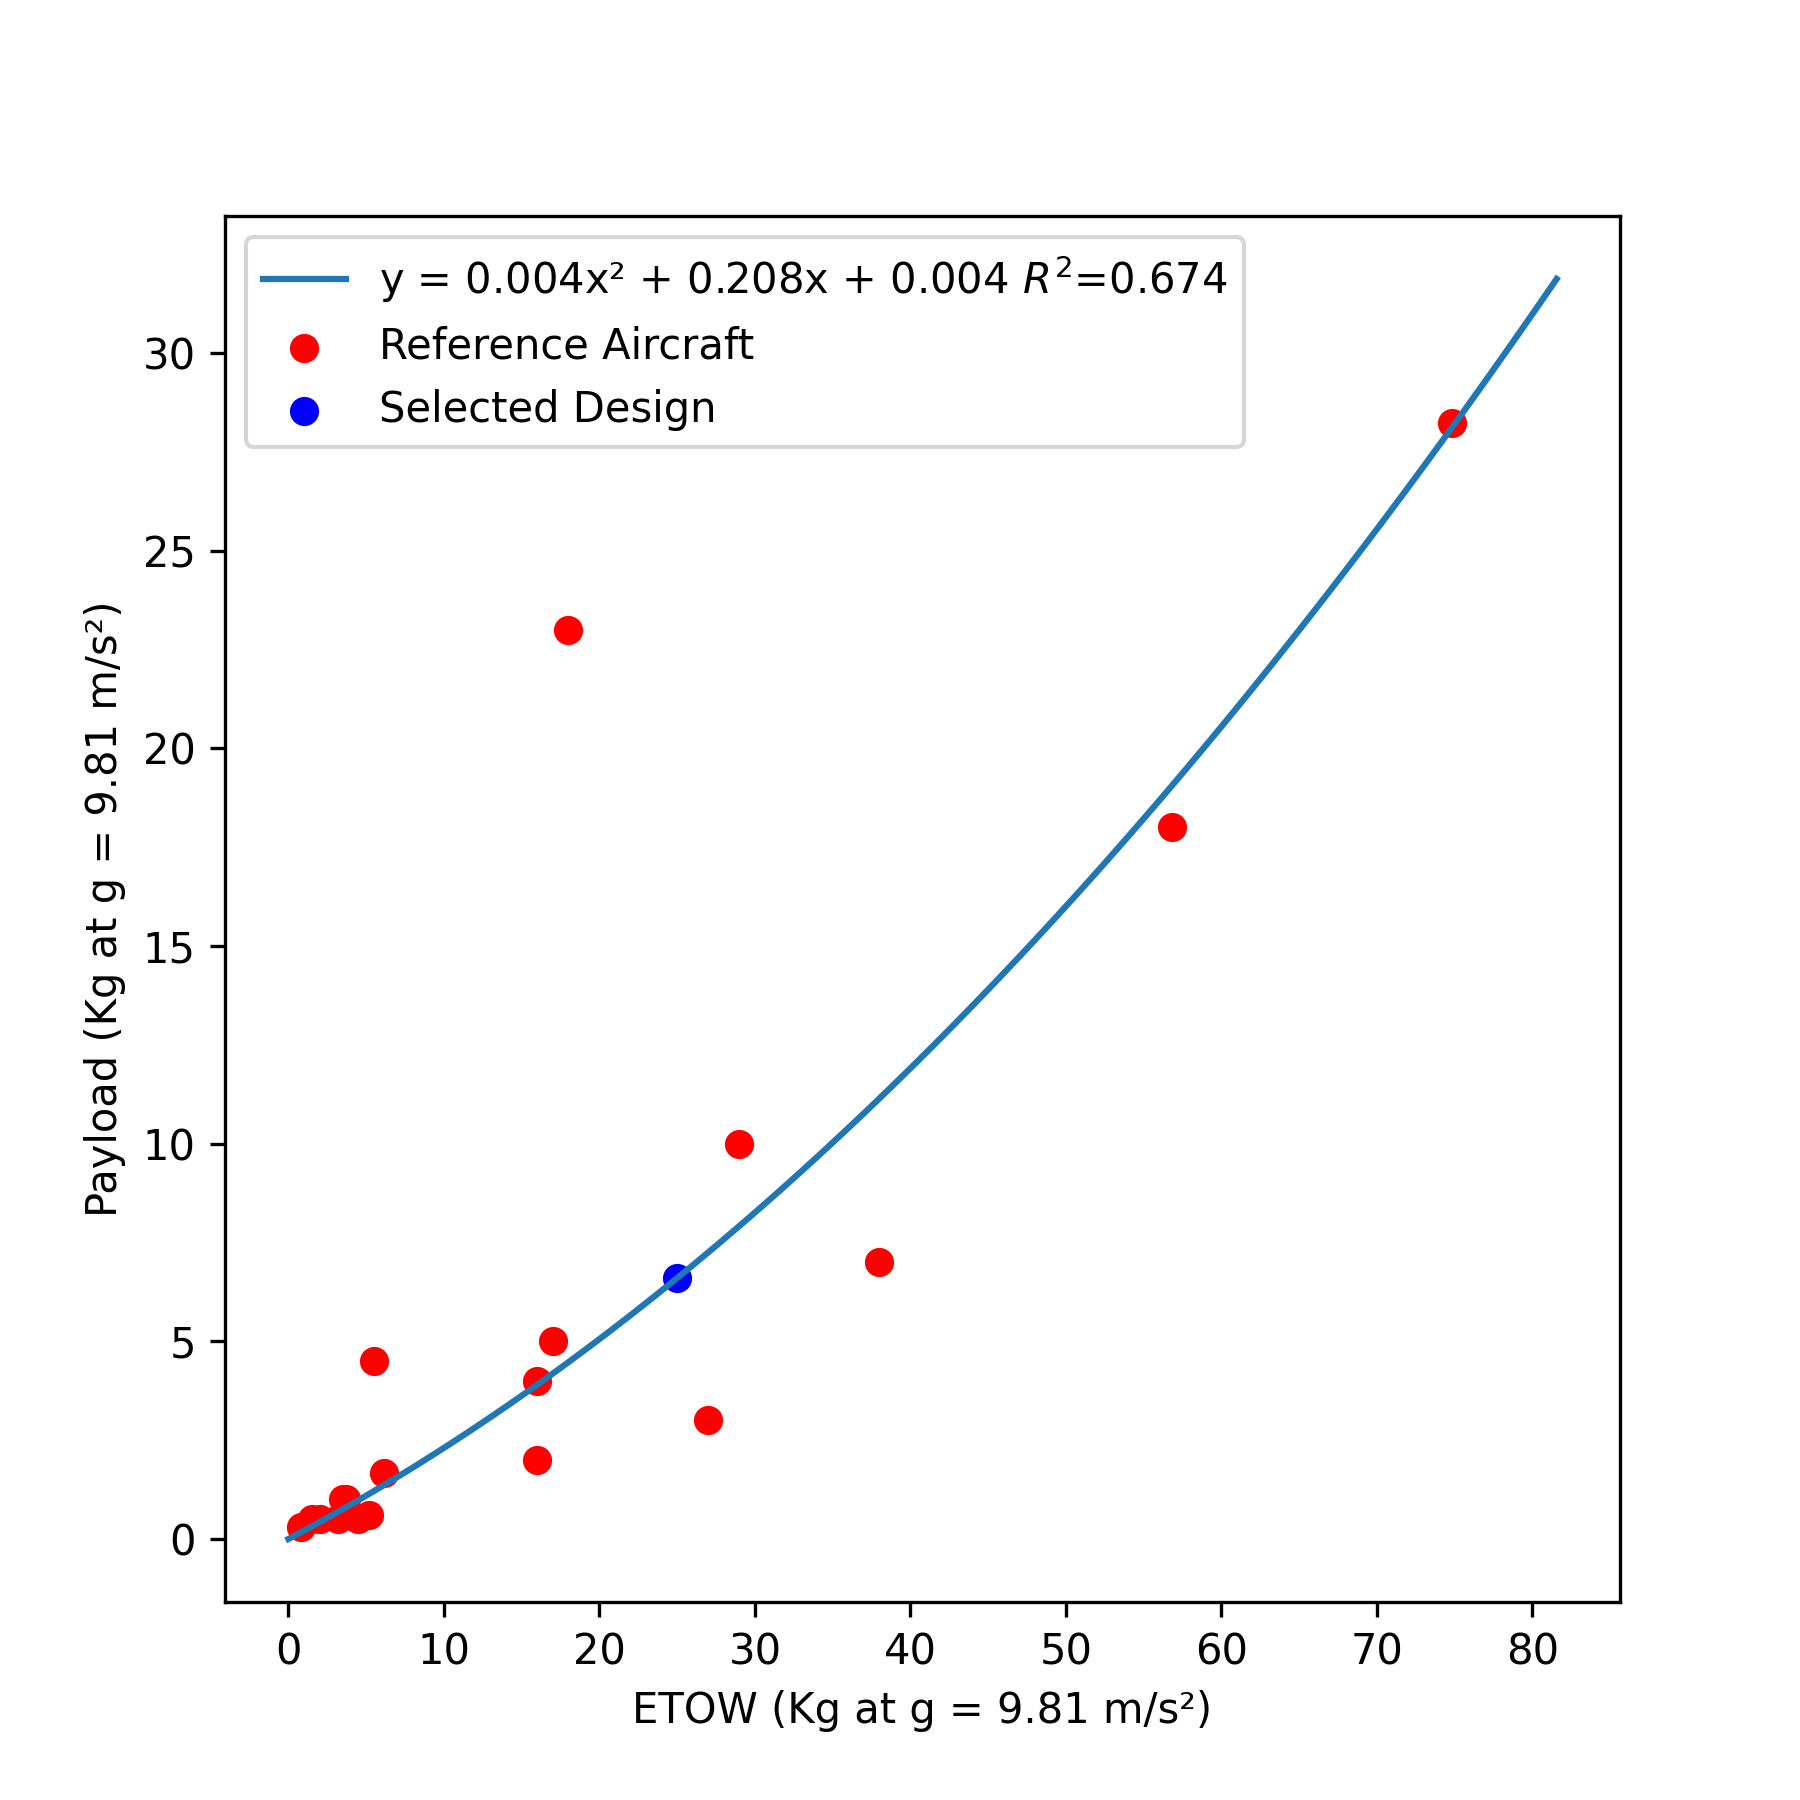
\includegraphics[width=6 in]{Figures/ETOW_vs_Payload.png} % Placeholder for technical drawings
		\caption{Payload weight as a function of ETOW presented as Kg at sea level}
		\label{fig:PayloadETOW}
	\end{figure}
	\newpage
	From this figure it can be estimated that with an ETOW of 25 Kg a payload of approximately 6.60 Kg can be carried. For the Heavy lift configuration 4 Kg of batteries can be sacrificed to effectively half the endurance but add 4 Kg of payload, totaling 10.60 Kg of payload.  From this the MTOW can be calculated to be 31.6 Kg. To compare this MTOW to other reference aircraft, ETOW was plotted against MTOW. 
	
	\begin{figure}[h!]
		\centering
		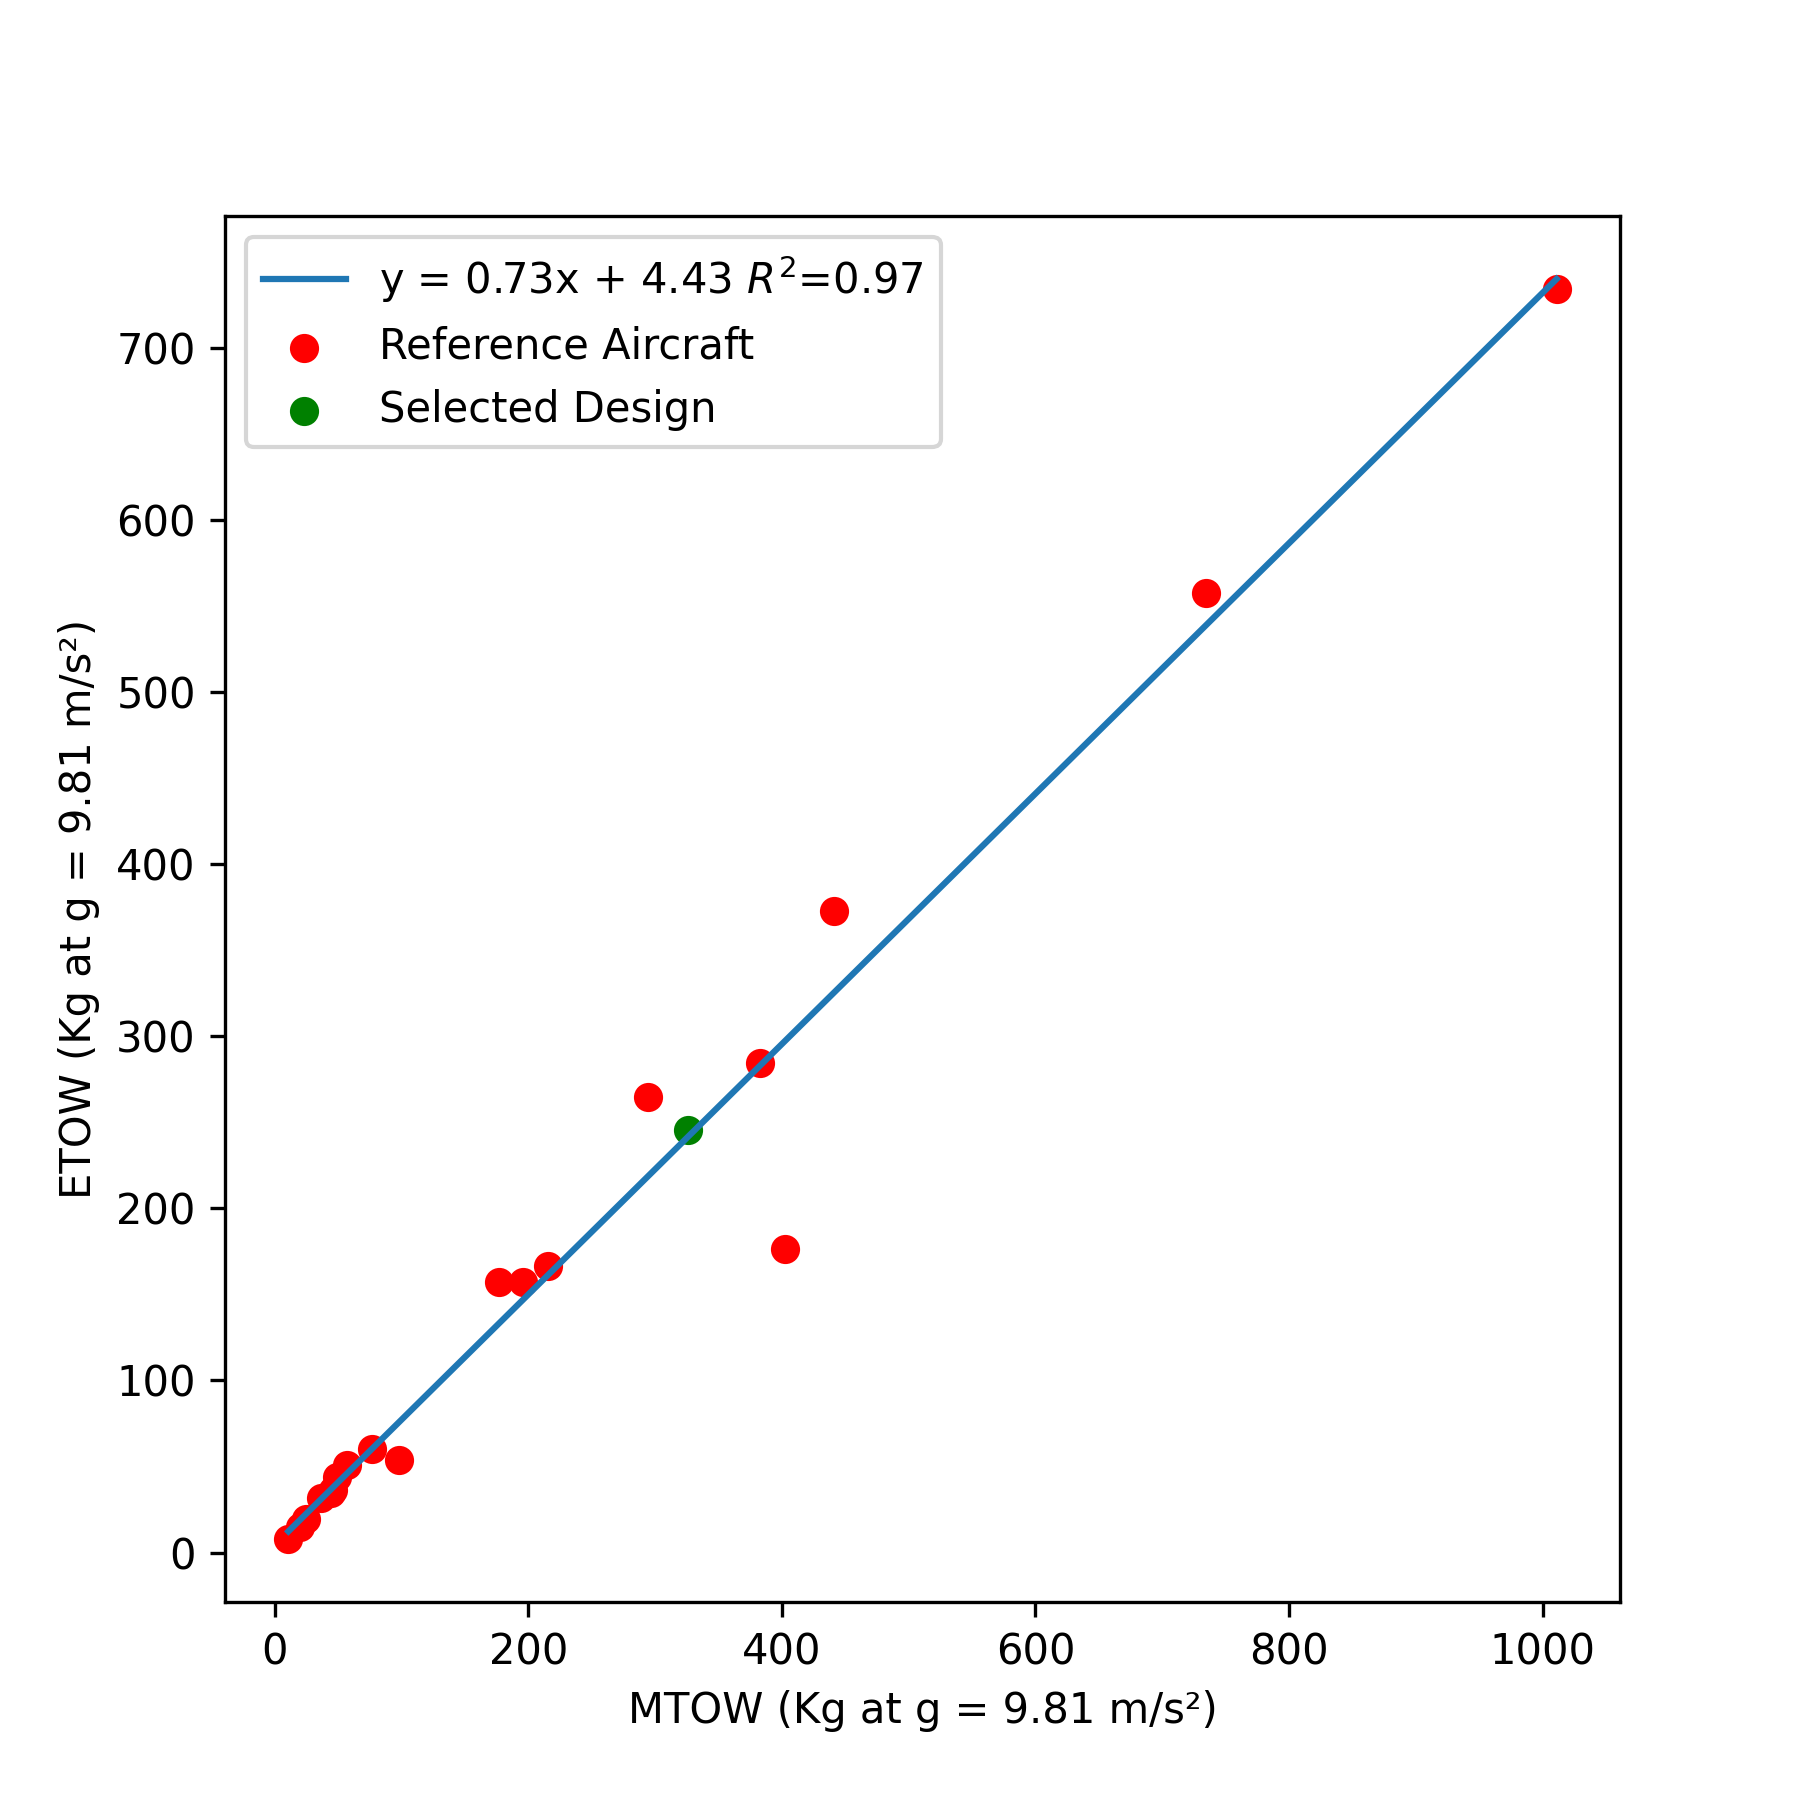
\includegraphics[width=6in]{Figures/MTOW_vs_ETOW.png} % Placeholder for technical drawings
		\caption{Payload weight as a function of ETOW presented as Kg at sea level}
		\label{fig:ETOWMTOW}
	\end{figure}
	
	\newpage

	\section{Determining the W/P-W/S Diagram}
	\subsection{Stall Sizing}
	$W/S$ limits for stall conditions can be calculated with the following equation:
	
	\begin{equation}
		\frac{W}{S}_{\text{stall}} = \frac{1}{2} \cdot \rho \cdot V_{\text{stall}}^2 \cdot C_{L_{max}}
	\end{equation}
	
	Max Coefficient of Lift $C_{lmax}$ is unknown but guesses can be made based on the $C_{L_{max}}$ of reference aircraft. For the design space of this aircraft the $C_{L_{max}}$ values range from 1.4 to 1.8. Cases for 1.4, 1.6 and 1.8 will be considered in this analysis. $V_{\text{stall}}$ can be estimated from the refrence aircraft. Most of the refrence aircraft have a stall speed of approximately 15 - 20 m/s. A worst - case estimation of  $V_{\text{stall}}$ = 20 m/s was selected for further analysis. 
	
	\subsection{Landing Sizing}
	A variety of factors are at play during the takeoff of an aircraft; these various factors are represented numerically using the take off parameter which is derived from the equation below.
	
	\begin{equation}
		TOP = \left(\frac{W}{S}\right)_{TO} \cdot \left(\frac{W}{P}\right)_{TO} \cdot \frac{1}{C_{L_{max}}} \cdot \frac{1}{\sigma}
	\end{equation}
	
	where $\sigma$ is the atmospheric density ratio, which is in this case 1 (for sea level take-off) 
	
	To empirically predict $TOP$, a relationship between $TOP$ and landing length was calculated with linear regression.
	
	\begin{figure}[h!]
		\centering
		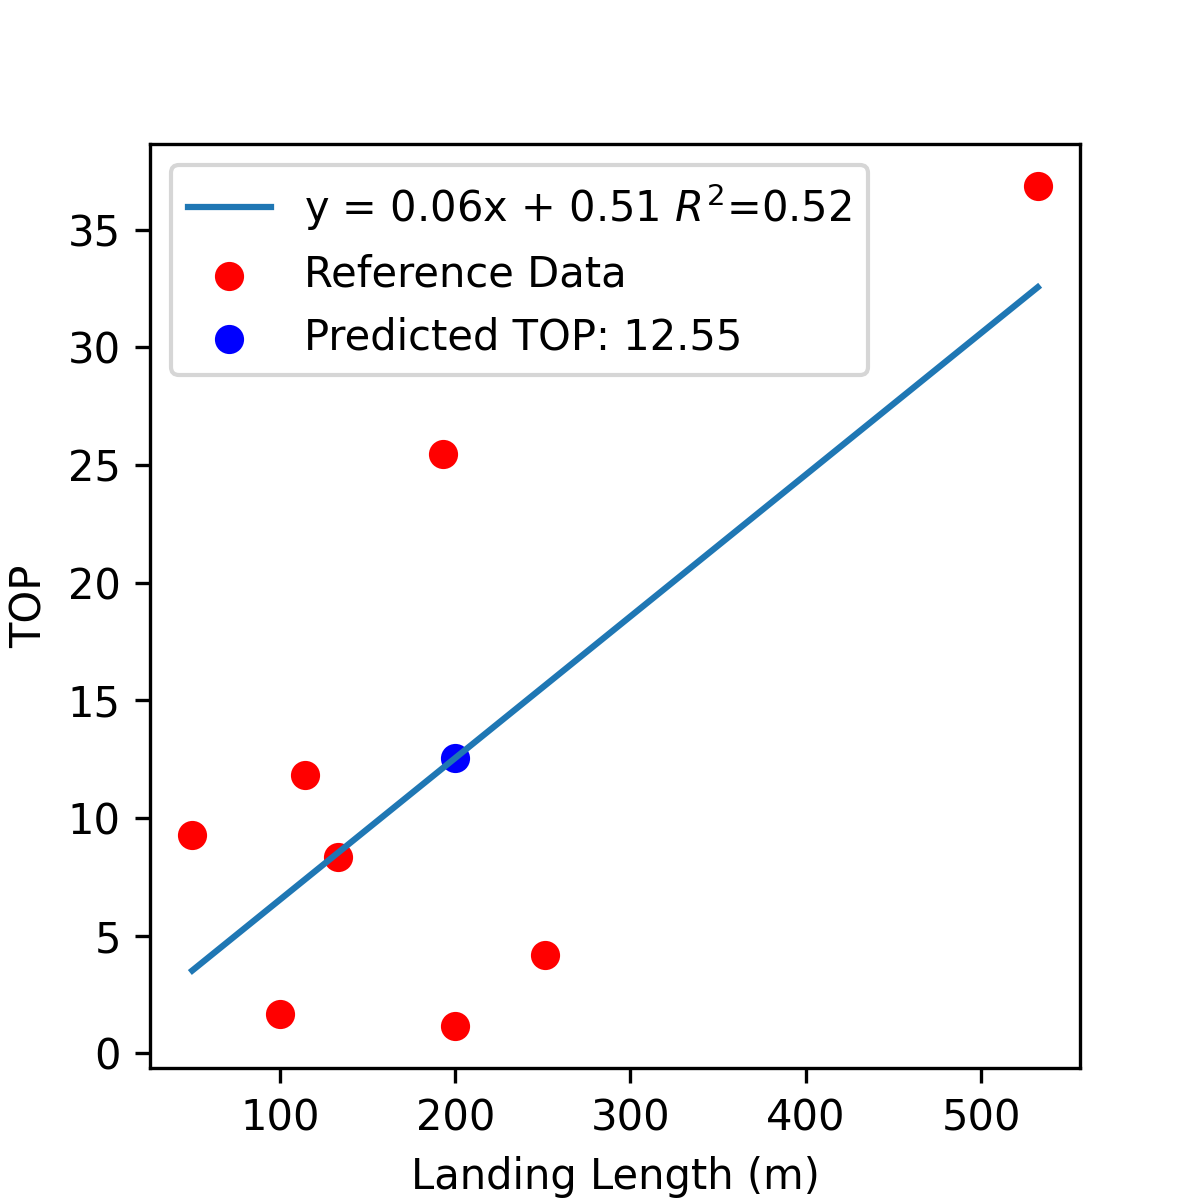
\includegraphics[width=6in]{Figures/TOP_vs_Landing_Length.png} % Placeholder for technical drawings
		\caption{TOP as a function of landing length}
		\label{fig:TOPLand}
	\end{figure}
	
	Though not exceptional an $R^2$ of .52 suggests this correlation is sufficient for first pass estimations. With a generous landing length of 200 meters selected a $TOP$ of 9.54 was predicted. With a known $TOP$, $(\frac{W}{P})_{TO}$ can be back calculated using the following equation, again this will be calculated for $C_{L_{max}}$ = 1.4, 1.6 and 1.8.
	
	\begin{equation}
		\left(\frac{W}{S}\right)_{TO} = \frac{C_{L_{max}} \cdot \rho \cdot \left(\frac{s}{0.5915}\right)}{2}
	\end{equation}
	\subsection{Take-Off Sizing}
	
	Take-off sizing as a function of $\left(\frac{W}{S}\right)^{-1}$ can be determined with the equation below:
	
	\begin{equation}
		\left(\frac{W}{P}\right) = \left(\frac{W}{S}\right)^{-1} \cdot TOP \cdot C_{L_{max}} \cdot \sigma
	\end{equation}
	

	\subsection{Climb Gradient Requirements}
	 The equation to compute $\frac{W}{P_{\text{br}}}$ is as follows:
	\begin{equation}
		\frac{W}{P_{\text{br}}} = \frac{\eta_p}{\sqrt{\frac{W}{S} \left( \frac{c}{V} + \frac{C_D}{C_L} \right)} \sqrt{\frac{2}{\rho C_L}}}
	\end{equation}
	
	To compute $\frac{W}{P_{\text{br}}}$ required for a given climb rate a few more variable need to be set or determined. In order to find reasonable climb performance requirements $c$, reference aircraft data was consulted. For this aircraft, a climb gradient of 5\% was selected. A strong climb gradient is not needed due to the mission requirements of this aircraft. A standard Propeller efficiency of 80\% was selected. For a high aspect, rectangular wing an Oswald efficiency of .7 was picked based on reference data. A $C_{D_0}$ of .035 was used based on reference data for fixed gear, small, single engine aircraft. $CD$ was calculated with the following equation:
	\begin{equation}
		C_D = C_{D_0} + \frac{C_L^2}{\pi \cdot A \cdot e}
	\end{equation}
	
	With this information, the climb rate data can be inserted into the $W/P$ – $W/S$ diagram. Since wing aspect ratio is unknown level curves at several aspect ratios will be plotted.
	
	\subsection{Climb Performance Requirement}
	The optimal climb performance requirements are found using the following equation:
	
	\begin{equation}
		\frac{W}{P_R} = \frac{\eta_p}{c + \sqrt{\left(\frac{W}{S}\right)} \cdot \sqrt{\frac{2}{\rho}} \cdot \left( \frac{1}{1.345 \cdot \left( (A \cdot e)^{0.75} \right) / C_{D_0}^{0.25}} \right)}
	\end{equation}
	
	With a moderate climb rate ($c$) of 5 m/s selected to match other UAV's in this design space, $	\frac{W}{P_R}$ curves can be generated at different aspect ratios. 

	\subsection{$W/P$ – $W/S$ diagram}
	
	With all of the information above the following diagram was able to be constructed. 
	
	\begin{figure}[h!]
		\centering
		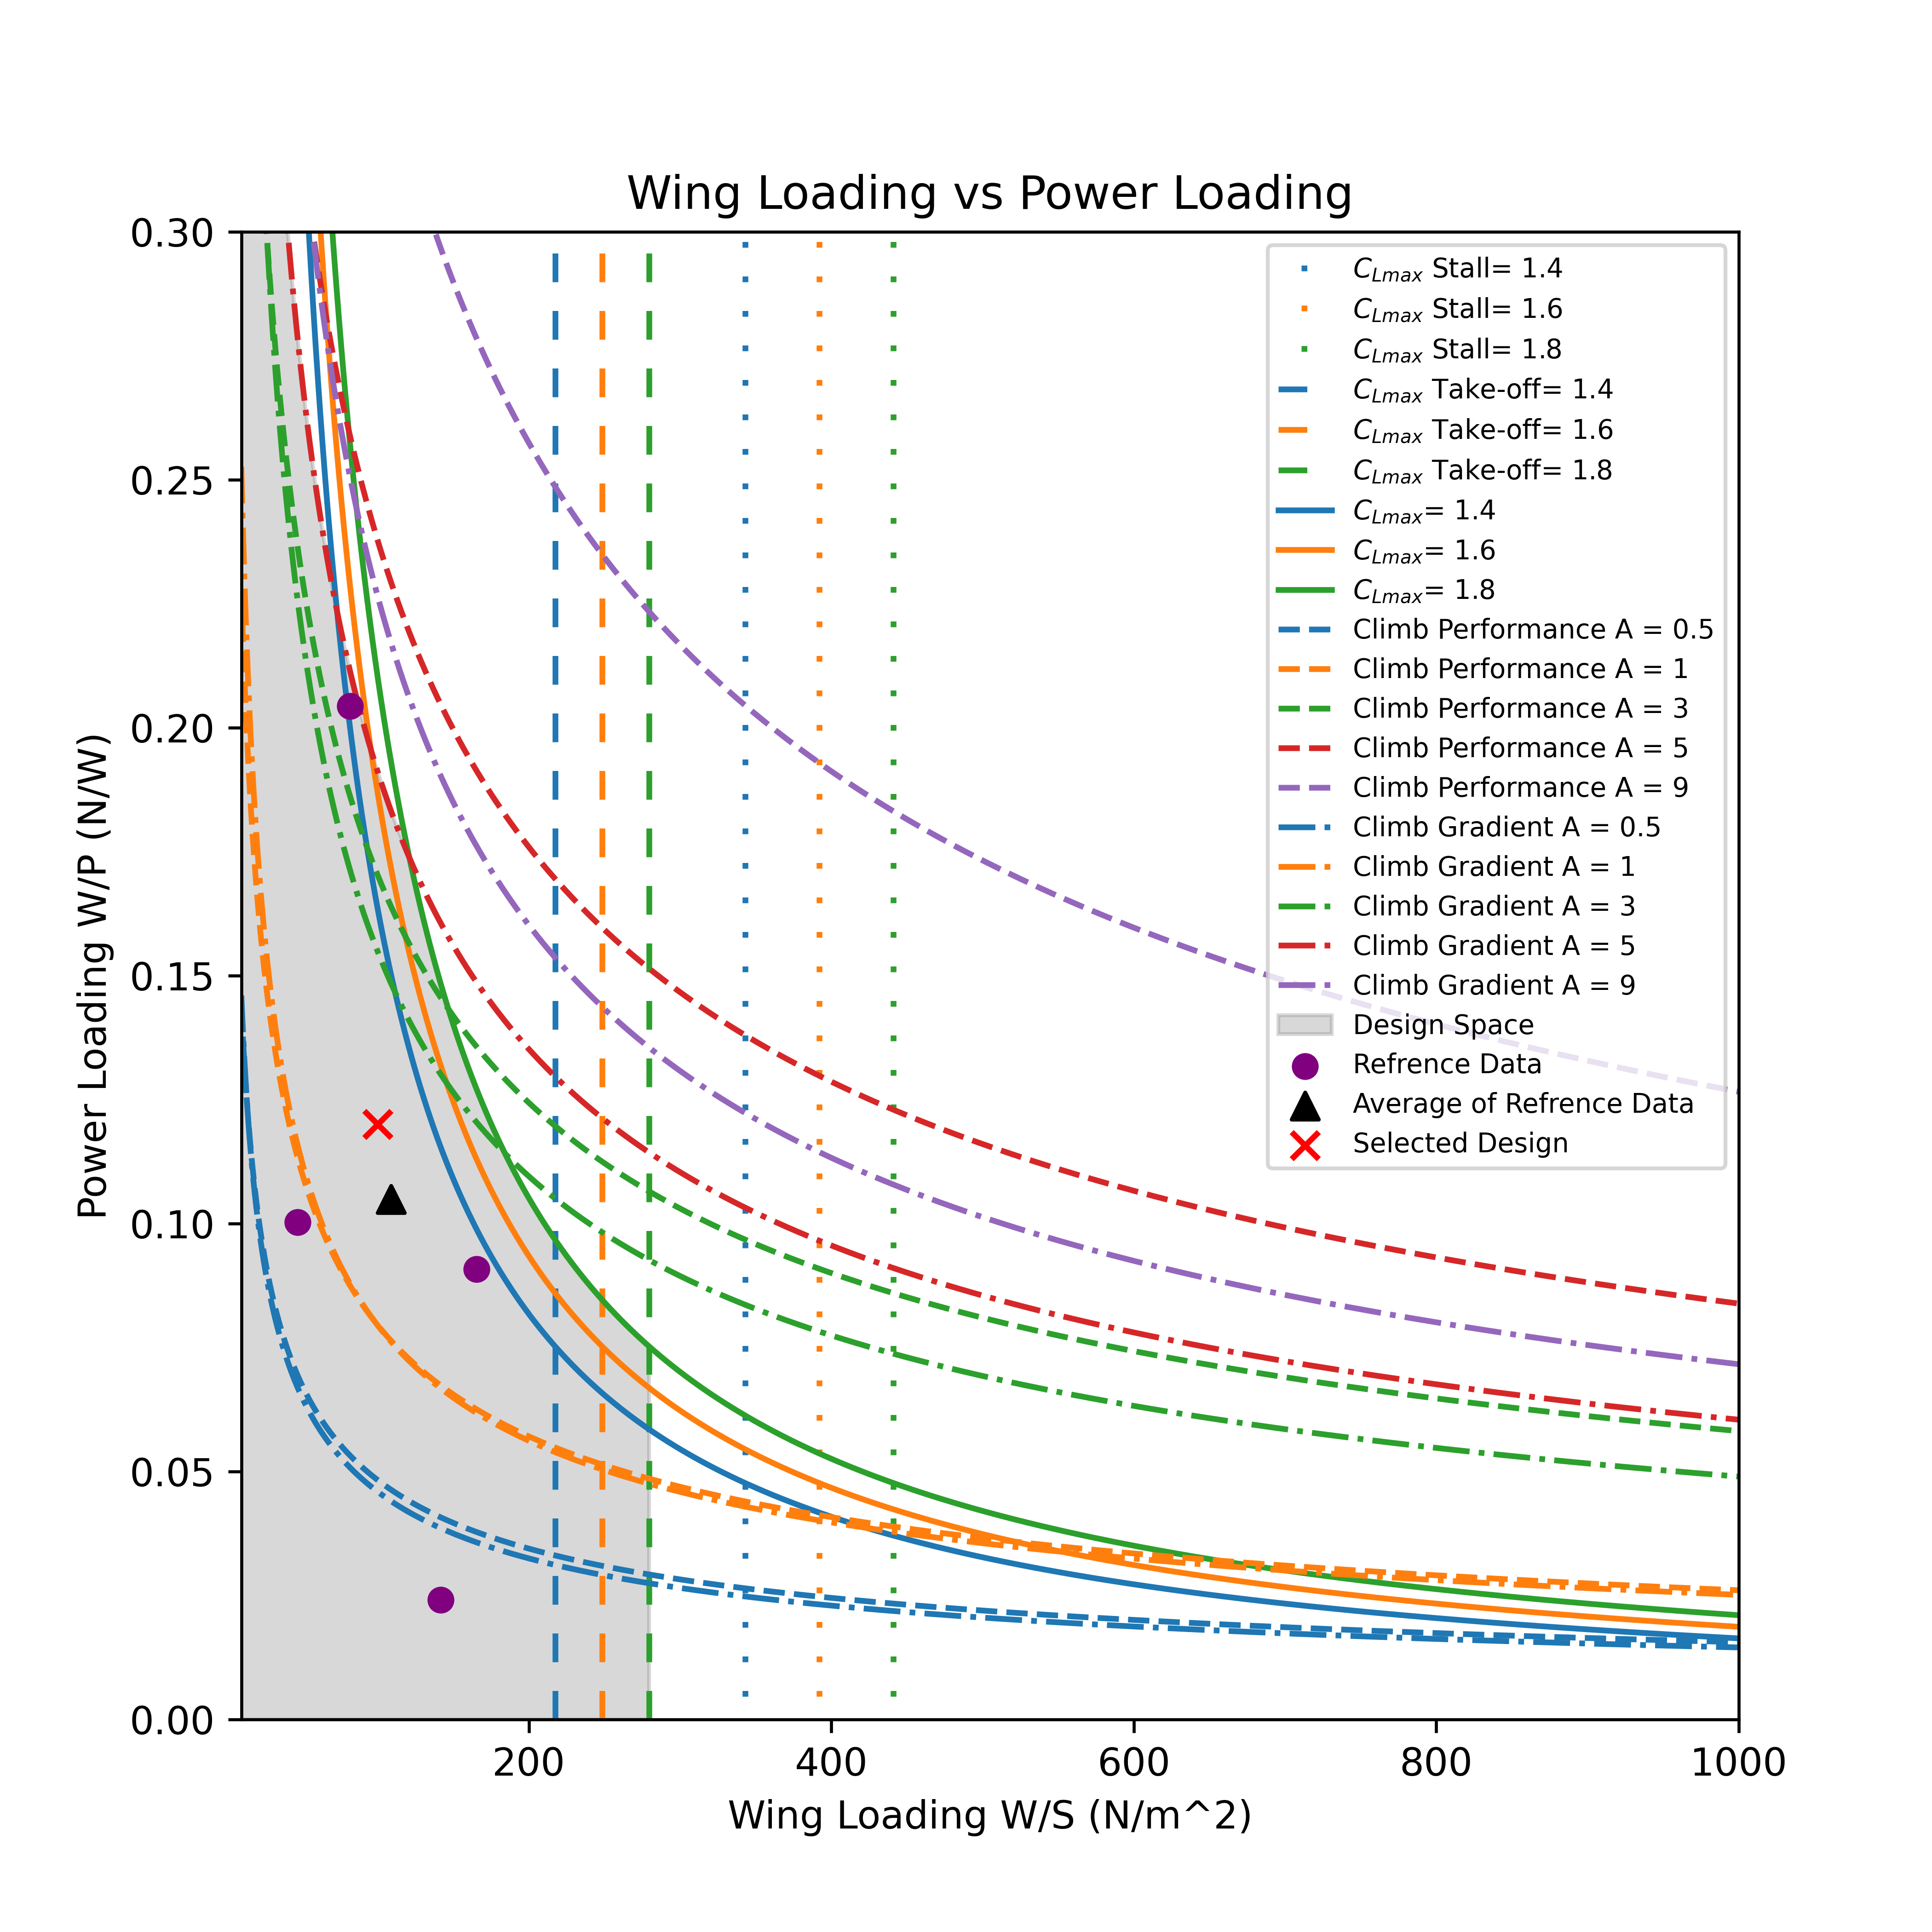
\includegraphics[width=7in]{Figures/Wing_Loading_vs_Power_Loading.png} % Placeholder for technical drawings
		\caption{$W/P$ – $W/S$ diagram with a highlighted design space outlining valid design conditions given the constraints set.}
		\label{fig:WPWSDiagram}
	\end{figure}
	
	The design space is bounded by the following conditions curves; climb gradient at an aspect ratio of 3, the maximum coefficient of lift of 1.8 curve, and the maximum coefficient of lift at take off of 1.8 curve. It can be observed that all listed reference aircraft fit within the design space, confirming the validity of the calculations. Not all of the necessary data to plot reference aircraft was able to be found, additionally non-electric aircraft were omitted as the different propulsion paradigm resulted in exceptionally different $W/P$ – $W/S$ points. This left only 4 reference aircraft to compare to, however the agreement with the calculations inspires sufficient confidence in the design. A conservative design near the reference craft was selected, with a $W/P$ of .12 and a $W/S$ of 100. A small wing loading was chosen particularity to minimize structural concerns allowing for more light weight wing construction in the future. 
	
	\subsection{Drag Polar}
	The Drag Polar of the aircraft can be calculated as a function of $C_L$ with the following equation:
	
	\begin{equation}
		C_D = C_{D_0} + \frac{C_L^2}{\pi \cdot A \cdot e}
	\end{equation}
	
	
	As this aircraft lacks passive or active high-lift devices only a clean configuration needs to be considered. Using all of the same values set above the following curve was generated, the L/D line was also calculated as the ratio of $C_L$ to $C_D$. The maximum lift to drag ratio was calculated to be 6.86.
	
	\begin{figure}[h!]
		\centering
		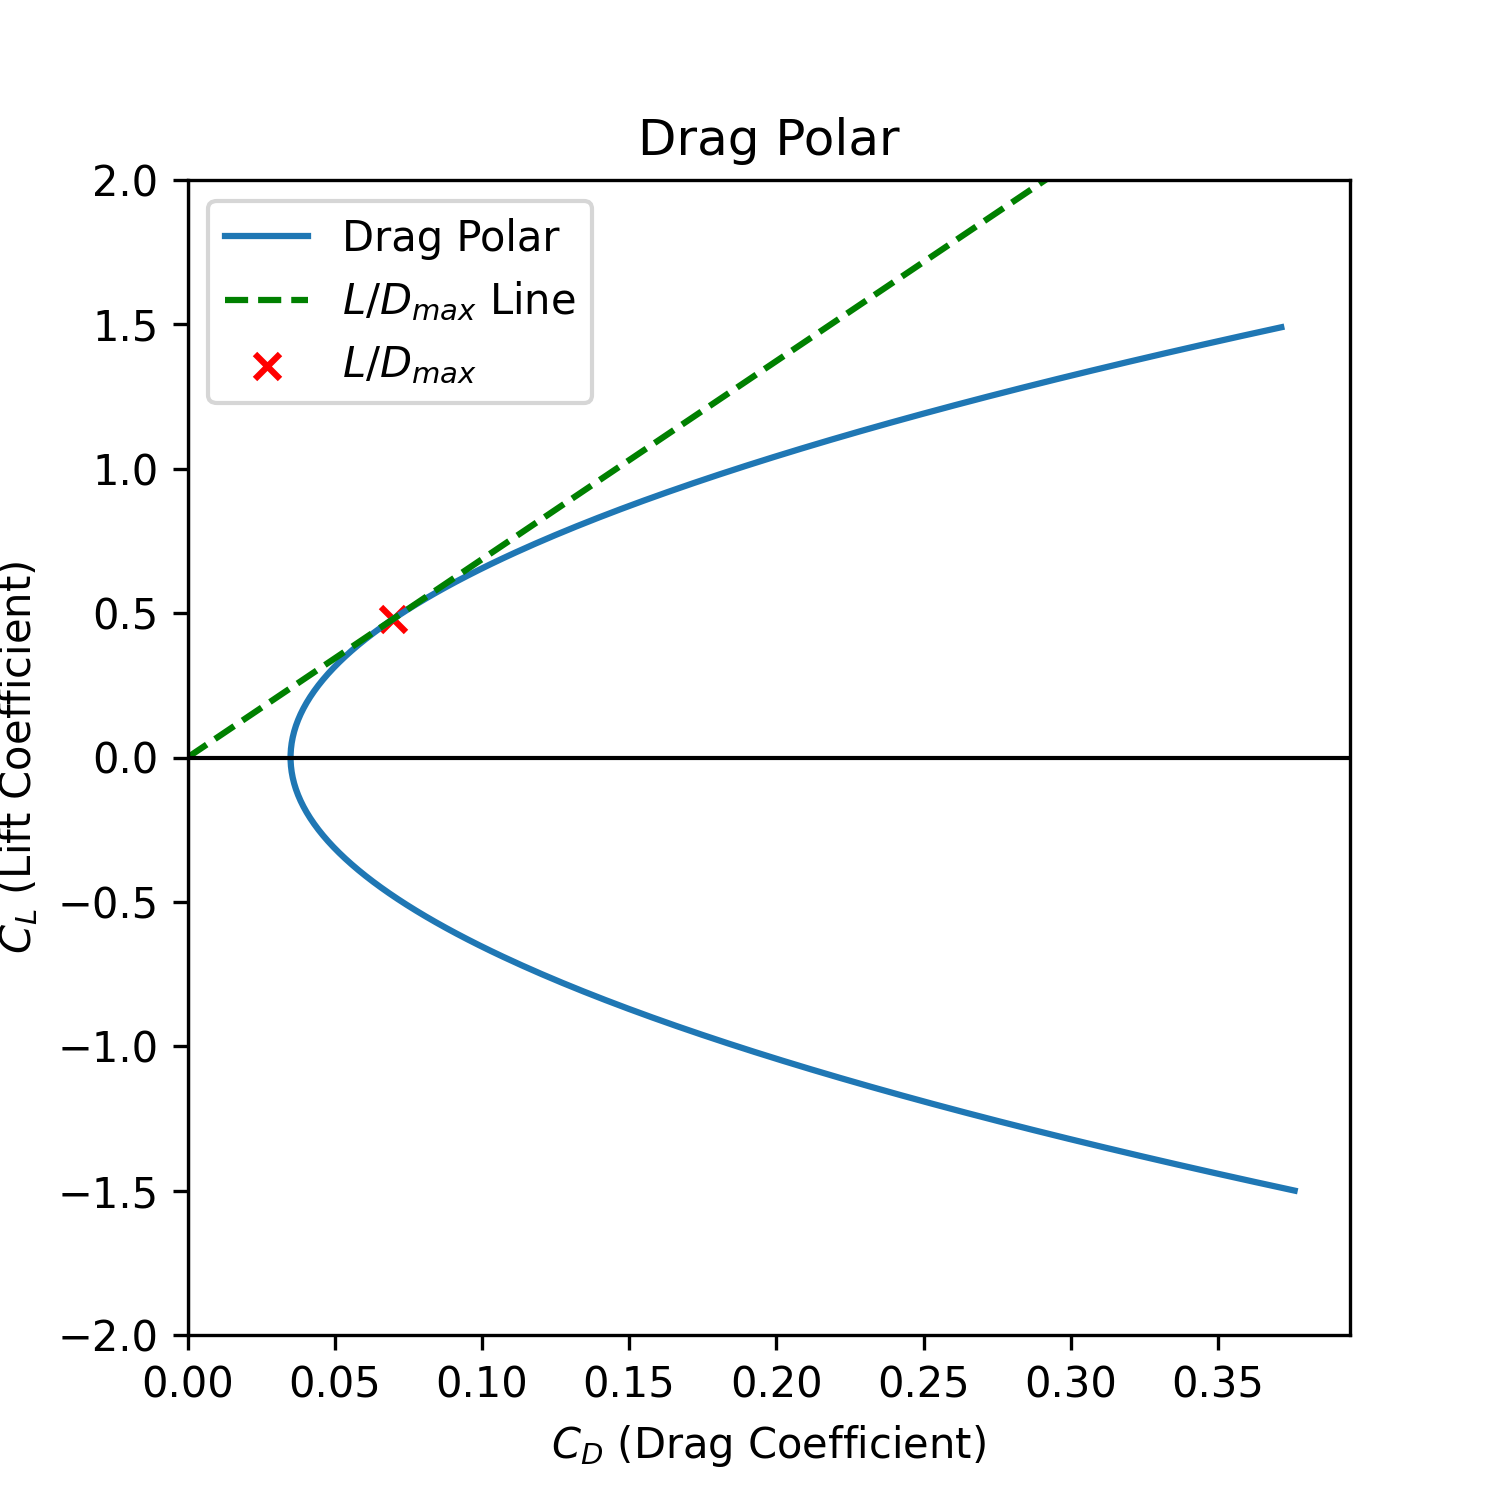
\includegraphics[width=5in]{Figures/Drag_Polar.png} % Placeholder for technical drawings
		\caption{The clean configuration drag polar diagram.}
		\label{fig:CDCL}
	\end{figure}
	\newpage
	\section{Propulsion Design}
	In the following chapter, the cruise, climb, and takeoff power required for flight will be calculated using the parameters found using the $W/P$ – $W/S$ diagram. Airworthiness requirements will also be explored in necessary depth.
	
	The max required power $P_R$ can be calculated simply from the $\left(\frac{W}{P}\right)_{\text{selected}}$ and the MTOW. With an MTOW of 33.23 Kg and a $\left(\frac{W}{P}\right)_{\text{selected}}$ of .12 N/W the max required power is approximately 2.717 KW. The required wing area $S$ can similarly be determined from $\left(\frac{W}{S}\right)_{\text{selected}}$ and MTOW. The calculated $S$ is approximately 3.26 $m^2$.
	
	\subsection{Engine Selection Criteria}
	Electric motors are most efficient at significantly less than 100\% throttle, most cannot sustain, without damage, more than 60\% throttle. Reference data from UAV electric motors suggest maximum efficiency is at around 40\% throttle. To optimize for endurance engines will be \textbf{over-sized} such that the ${P_R}$ is met at 40\% throttle.
	
	\subsection{Engine Selection from Market}
	To meet the $P_R$ requirement a series of motors from the T-Motor company were assessed.
	
	\begin{table}[h!]
		\centering
		\begin{tabular}{|c|c|c|c|c|}
			\hline
			\textbf{Motor} & \textbf{Power 40\% (W)} & \textbf{Max Power (W)} & \textbf{Current 40\% (A)} \\ \hline
			V13L KV65 24S  & 3390   & 18563  & 34.24  \\ \hline
			V10 KV160 12S  & 621.35 & 6084.92 & 134.53 \\ \hline
			V10L KV170 12S & 961.70 & 7673.50 & 20.29  \\ \hline
		\end{tabular}
		\caption{Motor Specifications at 40\% Throttle}
	\end{table}
	
	The V13L KV64 24S motor was selected for its high power output at 40\% throttle, with a diameter of 144.2 mm it can readily fit the fuselage. 
	
	\subsection{Engine Scaling}
	The engine can be scaled down to match the exact $P_R$ using the proportionality that follows:
	\begin{equation}
		P \propto D^3
	\end{equation}
	therefore:
	\begin{equation}
		D_{\text{scaled}} = D_{\text{ref}} \cdot \left( \frac{P_r}{W_{\text{ref}}} \right)^{\frac{1}{3}}
	\end{equation}
	
	the reference motor has a diameter of .144 m and a power of 3390 W. Plugging that into the equation yields:
	\begin{equation}
		D_{\text{scaled}} = .144 \cdot \left( \frac{2717}{3390} \right)^{\frac{1}{3}}
	\end{equation}
	
	$D_{\text{scaled}}$ is approximately equal to .124 m, the engine was scaled in diameter by 86.2\%. The weight of the original motor is 1.680 Kg since weight scales with the diameter of a cylinder squared the new weight would be $1.68 \cdot .862^2$ or 1.24 Kg. The estimated weight of the motor aligns closely with the original estimate of a 1 Kg motor. To accommodate the new engine weight a slightly reduced max payload of 6.36 can be set.  Due to practical manufacturing concerns the original motor would be used, however if this aircraft were to be mass produced the scaled motor may be economically justifiable to manufacture.
	
	\section{Range and Endurance}
	
	In this section, we will calculate the range and endurance of the electric UAV based on the battery capacity, power consumption, and flight parameters using modified Breguet equations. It should be noted that for this aircraft \textbf{no weight is lost in flight} this eliminates considerations of fuel fraction from the range and endurance calculations.
	
	\subsection{Range Calculation}
	
	The range of an electric aircraft can be determined using the following equation:
	
	\begin{equation}
		R = \left(\frac{C_b \cdot V_{\text{bat}}}{P_{\text{avg}}}\right) \cdot V
	\end{equation}
	
	Where:
	\begin{itemize}
		\item \(R\) is the range (in kilometers),
		\item \(C_b\) is the battery capacity (in ampere-hours, Ah),
		\item \(V_{\text{bat}}\) is the battery voltage (in volts, V),
		\item \(P_{\text{avg}}\) is the average power consumption (in watts, W),
		\item \(V\) is the true airspeed during cruise (in meters per second, m/s).
	\end{itemize}
	
	For our electric UAV, using a battery capacity of \(80 \, \text{Ah}\), a battery voltage of \(48 \, \text{V}\), and an average power consumption of \(1220 \, \text{W}\), the range can be calculated as follows:
	
	\[
	R = \left(\frac{80 \cdot 48}{1220}\right) \cdot 15 = 47.21 \, \text{km}
	\]
	
	Thus, the electric aircraft has an estimated range of 47.21 km under these conditions.
	
	\subsection{Endurance Calculation}
	
	The endurance of the electric UAV is calculated as:
	
	\begin{equation}
		E = \frac{C_b \cdot V_{\text{bat}}}{P_{\text{avg}}}
	\end{equation}
	
	Where:
	\begin{itemize}
		\item \(E\) is the endurance (in hours),
		\item \(C_b\) is the battery capacity (in ampere-hours, Ah),
		\item \(V_{\text{bat}}\) is the battery voltage (in volts, V),
		\item \(P_{\text{avg}}\) is the average power consumption (in watts, W).
	\end{itemize}
	
	For our electric UAV with the same values as above, the endurance is:
	
	\[
	E = \frac{80 \cdot 48}{1220} = 3.15 \, \text{hours}
	\]
	
	Therefore, the UAV's endurance is estimated to be 3.15 hours.
	
	\subsection{Power Required for Cruise}
	
	The power required during cruise is calculated using the equation:
	
	\begin{equation}
		P_{\text{cruise}} = \frac{C_D}{C_L} \cdot W \cdot V
	\end{equation}
	
	Where:
	\begin{itemize}
		\item \(P_{\text{cruise}}\) is the power required during cruise (in watts, W),
		\item \(C_D\) is the drag coefficient,
		\item \(C_L\) is the lift coefficient,
		\item \(W\) is the weight of the aircraft (in newtons, N),
		\item \(V\) is the cruise velocity (in meters per second, m/s).
	\end{itemize}
	
	Given the following values:
	\begin{itemize}
		\item \(C_D = 0.45\),
		\item \(C_L = 1.8\),
		\item \(W = 300 \, \text{N}\),
		\item \(V = 15 \, \text{m/s}\),
	\end{itemize}
	
	The power required for cruise is:
	
	\[
	P_{\text{cruise}} = \frac{0.45}{1.8} \cdot 300 \cdot 15 = 1220 \, \text{W}
	\]
	
	Thus, the power required during cruise is 1220 W.
	
	\subsection{Minimum Speed Calculation}
	
	The minimum speed required to keep the aircraft in the air is calculated using the equation:
	
	\begin{equation}
		V_{\text{min}} = \sqrt{\frac{2 \cdot W}{\rho \cdot S \cdot C_L}}
	\end{equation}
	
	Where:
	\begin{itemize}
		\item \(V_{\text{min}}\) is the minimum speed (in meters per second, m/s),
		\item \(W\) is the weight of the aircraft (in newtons, N),
		\item \(\rho\) is the air density (in kilograms per cubic meter, \(kg/m^3\)),
		\item \(S\) is the wing area (in square meters, \(m^2\)),
		\item \(C_L\) is the lift coefficient.
	\end{itemize}
	
	For an aircraft weight of \(300 \, \text{N}\), air density \(\rho = 1.225 \, \text{kg/m}^3\), wing area \(S = 3 \, \text{m}^2\), and lift coefficient \(C_L = 1.8\), the minimum speed is:
	
	\[
	V_{\text{min}} = \sqrt{\frac{2 \cdot 300}{1.225 \cdot 3 \cdot 1.8}} = 9.93 \, \text{m/s}
	\]
	
	Thus, the minimum speed required for the UAV to maintain flight is 9.93 m/s.
	


		
		\subsection{Proposed Improvements}

		
		To improve the specific energy consumption of electric motors, manufacturers can consider the following strategies, focusing on optimizing the motor design, enhancing power electronics, and improving thermal management.
		
		\subsubsection{1. Higher Efficiency Power Electronics (ESC)}
		
		The efficiency of an electric motor is closely tied to the performance of its power electronics, such as inverters and motor controllers, particularly the Electronic Speed Controller (ESC). Manufacturers could improve specific energy consumption by:
		
		\begin{itemize}
			\item \textbf{Silicon Carbide (SiC) and Gallium Nitride (GaN) Semiconductors:} 
			Using advanced materials such as SiC or GaN in ESCs allows for higher switching frequencies, lower energy losses, and improved thermal management. These semiconductors outperform traditional silicon-based systems, particularly under high load and high-temperature conditions, resulting in better overall efficiency.
			
			\item \textbf{Improved ESC Algorithms:} 
			Employing advanced control algorithms like Field-Oriented Control (FOC) or Direct Torque Control (DTC) can significantly optimize motor efficiency across varying loads. These algorithms allow for precise control over the motor's magnetic field and torque, minimizing energy losses and enhancing performance at all throttle levels.
			
			\item \textbf{ESC Cooling Systems:} 
			Integrating cooling mechanisms directly into ESCs can reduce thermal losses in high-performance applications. Liquid cooling or better heat sink designs can maintain the ESC at lower temperatures, reducing power losses due to overheating.
		\end{itemize}
		
		\subsubsection{2. Optimization of Motor Design (Core Materials and Windings)}
		
		Motor design plays a critical role in energy consumption. The following design optimizations can reduce losses and improve overall efficiency:
		
		\begin{itemize}
			\item \textbf{Advanced Core Materials:}
			Using high-performance materials such as soft magnetic composites (SMC) or amorphous metals in the stator and rotor cores reduces hysteresis and eddy current losses. These materials are more efficient than conventional ferromagnetic materials, particularly at higher speeds.
			
			\item \textbf{Optimized Windings:}
			Improving the design of the motor windings, such as using litz wire, can reduce resistance and skin effect losses. Additionally, optimizing the number of turns and the gauge of the wire in the windings can further minimize energy loss due to resistance (I²R losses).
			
			\item \textbf{Higher Pole Count:}
			Increasing the number of poles in the motor can provide greater torque at lower speeds, which enhances efficiency in applications where high-speed operation is not necessary.
		\end{itemize}
		
		\subsubsection{3. Improved Cooling and Thermal Management}
		
		As electric motors heat up during operation, their efficiency declines due to increased resistance in the windings and other losses. To mitigate this, manufacturers can improve thermal management:
		
		\begin{itemize}
			\item \textbf{Liquid Cooling Systems:}
			Implementing a liquid cooling system can significantly improve the thermal performance of an electric motor by keeping the operational temperature lower. This allows the motor to run at its optimal efficiency for extended periods and reduces the impact of heat-induced losses.
			
			\item \textbf{Thermally Conductive Insulation:}
			Using advanced thermally conductive materials in the motor's insulation helps dissipate heat more effectively. This prevents overheating of the windings and other components, improving motor durability and performance.
			
			\item \textbf{Enhanced Motor Housing Design:}
			A motor housing designed to improve airflow or incorporate heat sinks can also help to reduce the operating temperature, leading to more efficient energy use over longer periods.
		\end{itemize}
		
		
		In summary, manufacturers can significantly reduce specific energy consumption by focusing on:
		\begin{itemize}
			\item \textbf{Power electronics (ESCs)}: Utilizing high-efficiency semiconductors and advanced control algorithms to optimize motor performance.
			\item \textbf{Motor design optimizations}: Using advanced core materials and optimized windings to reduce energy losses.
			\item \textbf{Cooling systems and thermal management}: Implementing liquid cooling and advanced materials to keep the motor running efficiently at lower temperatures.
		\end{itemize}
		These improvements can result in longer operational ranges, increased endurance, and reduced overall energy consumption for electric UAVs and other electric motor applications.
		
		\newpage

			\begin{thebibliography}{99}
				
				% T-Motor References
				\bibitem{tmotor_v10}
				T-Motor, "V10 VTOL Motor," \url{https://store.tmotor.com/product/v10-vtol-motor.html}.
				
				\bibitem{tmotor_v10l}
				T-Motor, "V10L VTOL Motor," \url{https://store.tmotor.com/product/v10l-vtol-motor.html}.
				
				\bibitem{tmotor_v13l}
				T-Motor, "V13L VTOL Motor," \url{https://store.tmotor.com/product/v13l-vtol-motor.html}.
								
				% General Information
				\bibitem{faa}
				Federal Aviation Administration, "14 CFR Part 48," \url{https://www.faa.gov/air_traffic/publications/atpubs/aim_html/chap11_section_2.html}.
				
				% Aircraft References
				\bibitem{applied_aeronautics}
				Applied Aeronautics, "Applied Aeronautics," \url{https://www.unmannedsystemstechnology.com/company/applied-aeronautics/}.
				
				\bibitem{uavos_sat_i}
				UAVOS, "SAT-i," \url{https://www.uavos.com/products/fixed-wing-uavs/sat-i/}.
				
				\bibitem{uavos_sitaria_e}
				UAVOS, "SITARIA E," \url{https://www.uavos.com/products/fixed-wing-uavs/sitaria-e/}.
				
				\bibitem{uavos_borey_10}
				UAVOS, "BOREY 10," \url{https://www.uavos.com/products/fixed-wing-uavs/borey-10/}.
				
				\bibitem{aeromapper}
				Aeromapper, "Aeromapper," \url{https://www.directindustry.com/prod/aeromapper/product-182310-1802491.html}.
				
				\bibitem{insitu_scaneagle}
				Insitu, "ScanEagle Product Card," \url{https://www.insitu.com/wp-content/uploads/2020/12/ScanEagle_ProductCard_DU120320.pdf}.
				
				\bibitem{eos}
				EOS Technology, "Strix 300," \url{https://www.eos-technologie.com/strix-300/}.
				
				\bibitem{c_astral}
				C-Astral, "Unmanned Aircraft Systems," \url{https://pdf.directindustry.com/pdf/c-astral/unamanned-aircraft-systems/182250-945853.html#open2113345}.
				
				\bibitem{quantum_systems}
				Quantum Systems, "Trinity PRO," \url{https://quantum-systems.com/trinity-pro/}.
				
				\bibitem{geo_matching_dt26x}
				Geo-Matching, "DT26X LiDAR," \url{https://geo-matching.com/products/dt26x-lidar}.
				
				\bibitem{direct_industry_delair}
				DirectIndustry, "Delair," \url{https://www.directindustry.com/prod/delair/product-108459-1800225.html}.
				
				\bibitem{geo_matching_bramor_sar}
				Geo-Matching, "C-Astral Bramor SAR," \url{https://geo-matching.com/products/c-astral-bramor-sar}.
				
				\bibitem{aeromao_vtnaut}
				Aeromao, "VTNAUT," \url{https://aeromao.com/products/vtnaut/}.
				
				\bibitem{aeroexpo}
				AeroExpo, "UAV Factory Ltd. Europe," \url{https://www.aeroexpo.online/prod/uav-factory-ltd-europe/product-174156-793.html}.
				
				\bibitem{griffon_outlaw}
				Griffon Aerospace, "Outlaw G2," \url{https://www.griffonaerospace.com/products/outlaw-g2/}.
				
				\bibitem{unmanned_systems_pd1}
				Unmanned Systems Technology, "PD-1 Fixed Wing UAV," \url{https://www.unmannedsystemstechnology.com/wp-content/uploads/2016/06/PD-1-Fixed-Wing-UAV.pdf}.
				
				\bibitem{c_astral_bramor_c4eye}
				C-Astral, "Bramor C4Eye," \url{https://www.c-astral.com/en/unmanned-systems/bramor-c4eye}.
				
				\bibitem{satuav}
				Satuav, "Glider Drone Runway Drone," \url{https://www.satuav.com/glider-drone-runway-drone/long-endurance-fixed-wing-drone.html}.
				
				\bibitem{uav_systems_talon_gt}
				UAV Systems International, "Talon GT Drone," \url{https://uavsystemsinternational.com/products/talon-gt-drone}.
				
				\bibitem{uav_systems_skywalker}
				UAV Systems International, "Skywalker Drone," \url{https://uavsystemsinternational.com/products/skywalker-drone}.
				
				\bibitem{ua_sp}
				UA SP, "Altavian," \url{https://www.ua-sp.com/altavian}.
				
				\bibitem{insitu_integrator}
				Insitu, "Integrator," \url{https://www.insitu.com/products/integrator}.
				    % USC PowerPoint Slides
				\bibitem{usc_prelim_sizing1}
				University of South Carolina, "Preliminary Sizing 1," AESP 415 Lecture Notes, Version 3, \url{https://www.example.com/AESP415_001_06-PreliminarySizing1_V3}.
				
				\bibitem{usc_prelim_sizing2}
				University of South Carolina, "Preliminary Sizing 2," AESP 415 Lecture Notes, Version 3, \url{https://www.example.com/AESP415_001_06-PreliminarySizing2_V3}.
				
				
				
							
			
		\end{thebibliography}
		
		\newpage
		


			\begin{figure}[h!]
				\centering
				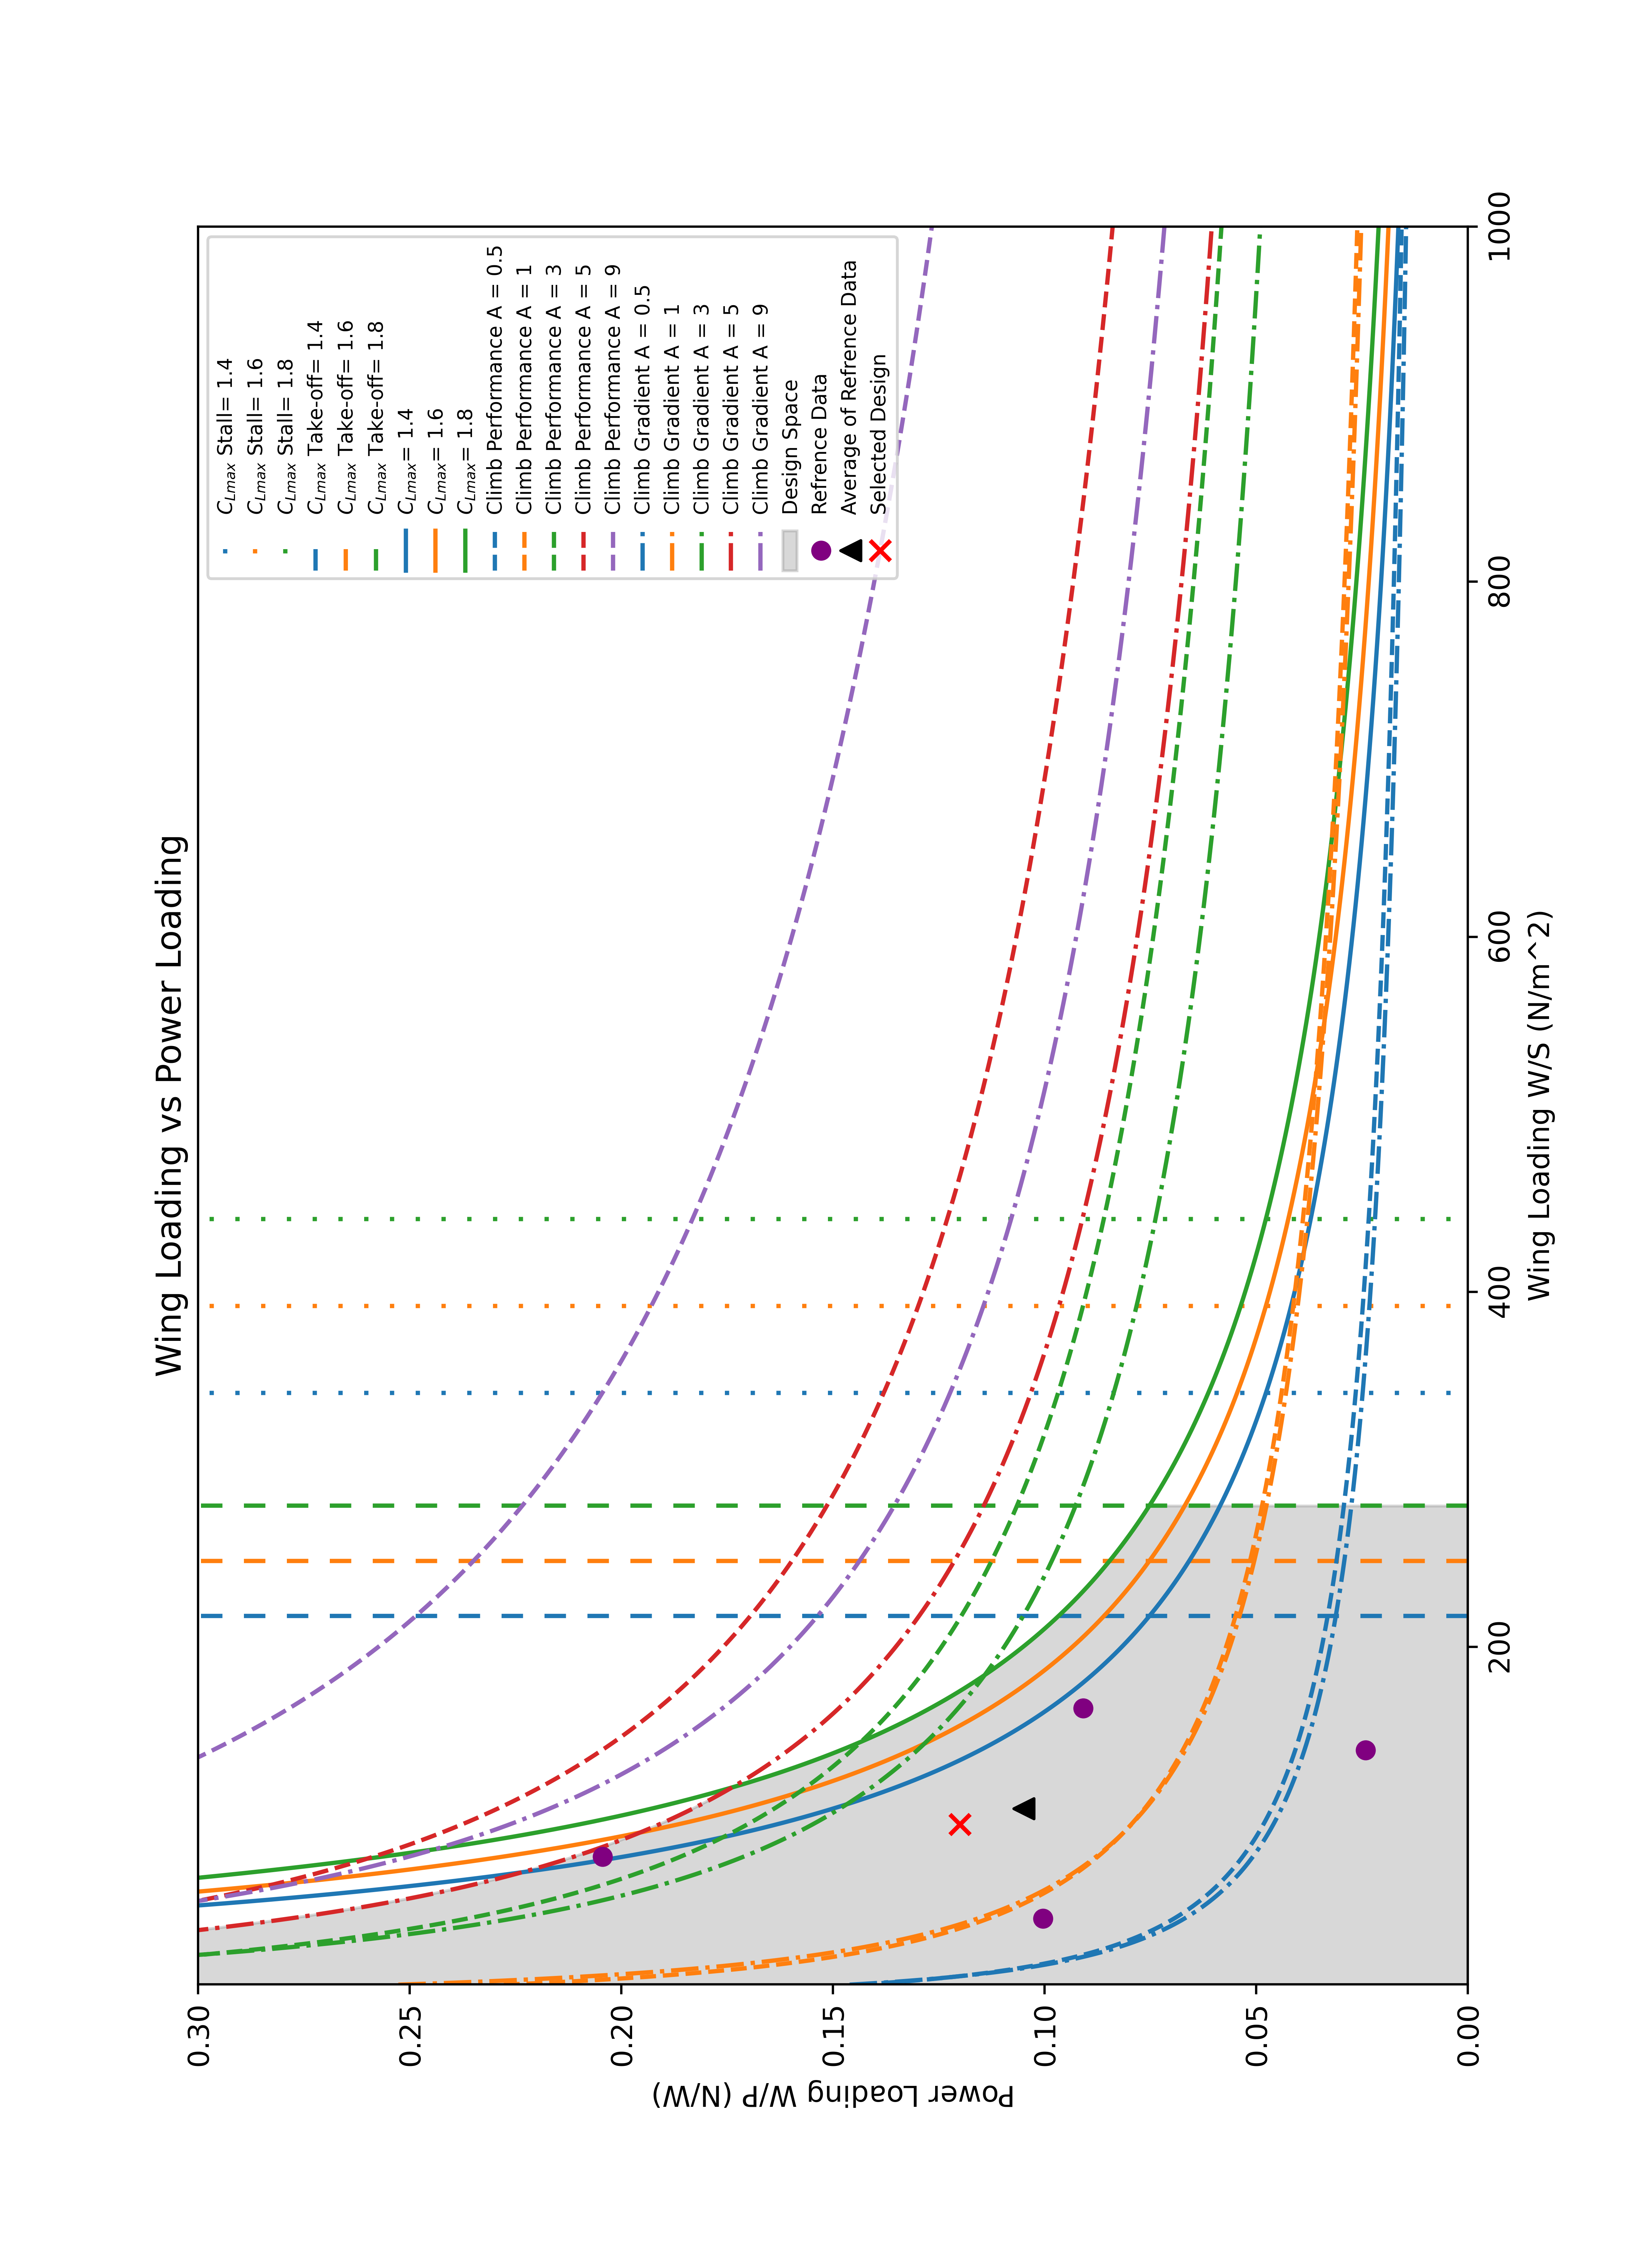
\includegraphics[width=7in]{Figures/Wing_Loading_vs_Power_Loading_appendix.png}  % Replace with your figure file
				\caption{ \textbf{Appendix B} larger W/S - W/P Figure}
				\label{fig:fullpage}
			\end{figure}

		\newpage
		
		\section*{Appendix A: Power and Propulsion Aircraft Parameters Table}
		\begin{table}[h!]
			\centering
				\caption{Current Aircraft Propulsion and Flight Parameters for the UAV }
			\begin{tabular}{|l|l|l|l|}
				\hline
				\textbf{Symbol}    & \textbf{Parameters}                  & \textbf{Value}    & \textbf{Unit} \\ \hline
				\multicolumn{4}{|l|}{\textbf{Wing Characteristics}}                                                        \\ \hline
				
				b                 & Wing span                             & 3.26              & m²            \\ \hline
				A                 & Aspect ratio                          & 3                 & \_             \\ \hline
				\multicolumn{4}{|l|}{\textbf{Weights and Loadings}}                                                          \\ \hline
				$W_{TO}$            & Maximum takeoff weight                & 31.6              & kg            \\ \hline
				$W_{OE}$            & Operational empty weight              & 25.0              & kg            \\ \hline
				$W_{Payload}$       & Payload weight                        & 6.60              & kg            \\ \hline
				$W_{Battery1}$      & Battery weight 					       & 8.00              & kg            \\ \hline
				W/S               & Wing loading                          & 100               & N/m²          \\ \hline
				P/W               & Power-to-weight ratio                 & 0.086             & kW/kg         \\ \hline
				\multicolumn{4}{|l|}{\textbf{Flight Parameters}}                                                           \\ \hline
				$V_{cruise}$        & Cruise speed                          & 15         & m/s           \\ \hline
				$h_{cruise}$        & Cruise altitude                       & 122               & m             \\ \hline
				Endurance         & Endurance                             & 3.15              & hours         \\ \hline
				Range             & Range                                 & 47.21             & km            \\ \hline
			\end{tabular}

		\end{table}


		
	\end{document}
